\chapter{Appendix: Simulation Depth Camera Misalignment}\label{chapter:appendix:gz_depth_camera}

When first attempting to implement a depth camera as ground truth I noticed a misalignment of the depth camera FOV and a normal camera's image. This was the case even with equal camera parameters:


\begin{figure}[ht]
    \centering
    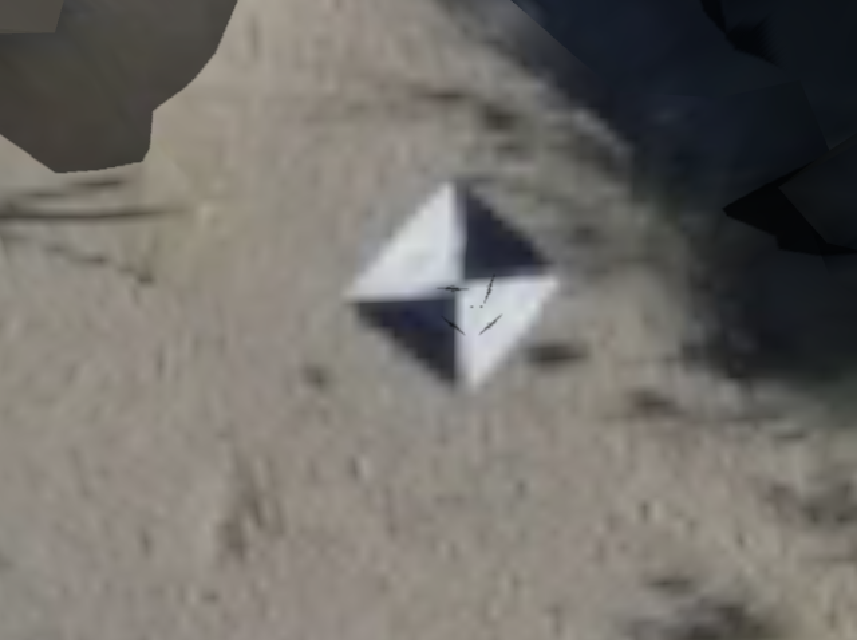
\includegraphics[scale=0.4]{images/preparation/GT_error_sim.png}
    \caption{Simulation Reference}
    \label{fig:GT_error_sim}
\end{figure}
\begin{figure}
    \centering
    
\includegraphics[scale=0.4]{images/preparation/GT_error_GT.png}
    \caption{GT depth image with wrong calibration}
    \label{fig:GT_error_GT} %TODO Use color coded image
\end{figure}

\clearpage %HERE

Looking at \cref{fig:GT_error_sim} and \cref{fig:GT_error_GT} the error looks like a simple translation error or is even hard to see at all. Focus for instance on the edge of the canapé in the top left. When comparing the extrinsic parameters of the cameras, they were perfectly aligned. 
Later tests showed however, that there was an actual error in the Gazebo Garden source code.\footnote[1]{For more footage on this see \cref{chapter:appendix:gz_depth_camera}} No matter what camera parameters were passed, the depth camera had the same FOV. 

Thanks to my friend and colleague Simone Nascivera, this bug could be fixed.